\documentclass[twocolumn, longbibliography]{revtex4-2}

\usepackage{amsmath}
\usepackage[dvipsnames]{xcolor}
\usepackage{hyperref}
\hypersetup{
	colorlinks=true,
	linkcolor=blue,   
	urlcolor=blue,
}
\usepackage{graphicx}
\usepackage{tikz}

\newcommand{\note}[1]{\textcolor{red}{#1}}
\newcommand{\outline}[1]{\textcolor{Plum}{#1}}
\newcommand{\todo}[1]{\textcolor{orange}{#1}}
\newcommand{\charlie}[1]{\textcolor{TealBlue}{#1}}
\newcommand{\RN}[1]{\textcolor{TealBlue}{#1}}
\newcommand{\op}[1]{\mathcal{O}^{(#1)}}
\newcommand{\nn}{\nonumber\\}
\newcommand{\goesto}{\rightarrow}
\renewcommand{\max}{\text{max}}
\newcommand{\eff}{\text{eff}}
\newcommand{\cl}{\text{cl}}
\newcommand{\q}{\text{q}}
\newcommand{\half}{\frac{1}{2}}

\begin{document}
	
\title{Spontaneous breaking of multipole symmetries}
\author{Charles Stahl}
\author{Rahul Nandkishore}
\affiliation{Department of Physics and Center for Theory of Quantum Matter, University of Colorado Boulder, Boulder CO 80309, USA}

	
\begin{abstract}
Multipole symmetries are of interest both as a window on fracton physics and as a crucial ingredient in realizing new universality classes for quantum dynamics. Here we address the question of whether and when multipole symmetries can be {\it spontaneously broken} in thermal equilibrium. We derive generalized Mermin-Wagner arguments for the total or partial breaking of multipolar symmetry groups and generalized Imry-Ma arguments for the robustness of such multipolar symmetry breaking to disorder. We present both general results and explicit examples. Our results should be directly applicable to quantum dynamics with multipolar symmetries and also provide a useful stepping stone to understanding the robustness of fracton phases to thermal fluctuations, quantum fluctuations, and disorder. 
\end{abstract}
	
\date{\today}
	
\maketitle

\section{Introduction}

Hamiltonians invariant under polynomial symmetry transformations conserve not only charge, but also various multipole moments of charge. Such `multipolar' symmetries are known to offer a robust route to ergodicity breaking \cite{PPN, KHN, Sala, Moudgalya, SLIOM, commutant}, and also to exotic universality classes of quantum dynamics \cite{Iaconis1, GLN, nonabelian, glorioso, MKH, Feldmeier, Iaconis2}. They are known to arise in `fracton' phases of quantum matter \cite{Chamon, Haah, VHF1, VHF2, NH, PretkoRadzihovsky}, the key dynamical properties of which are known to descend from conservation laws on multipole moments of charge \cite{Pretko1, BB,  Gromov2019}. They are also known to arise (in a prethermal sense) in various ultracold atom platforms \cite{KHN, Bakr, Aidelsburger}. There are thus multiple reasons for thinking about systems with multipolar symmetries. However, just because a symmetry is present in the {\it Hamiltonian} does not mean that it will be present in the {\it state}; there is always the possibility of spontaneous symmetry breaking (SSB). 

For conventional symmetries, there exist general theorems which constrain the settings in which SSB can occur. In clean systems, the relevant theorem is due to Mermin and Wagner \cite{MerminWagner}, and involves the physics of (thermal or quantum) fluctuations of the Goldstone modes associated with SSB, whereas in disordered systems the key results are due to Imry and Ma \cite{ImryMa, Vojta2013}, and also Aizenman and Wehr \cite{Aizenman}, and involve the physics of order parameter deformation for local alignment with disorder. Multipolar symmetries, however, allow for a much richer pattern of possible symmetry breakings (including breaking some but not all of the multipolar symmetries), and the analogous theorems have not yet been derived, except in the special case of isotropic clean systems with total breaking of the symmetry \cite{Griffin2013Multi}.

In this work, we place generalized Mermin-Wagner and Imry-Ma constraints on the total and/or partial breaking of multipolar symmetries, in both clean and disordered systems. Along the way we also discuss the exotic Goldstone modes associated with total or partial SSB of multipolar symmetries. We will also provide explicit models of multipole symmetry breaking, to give intuition for these unusual forms of SSB. 

Throughout, we consider only multipole groups where the underlying internal group is continuous and abelian. For concreteness, we will say it is $U(1)$. Multipole groups with a nonabelian underlying symmetry suffer a cascade effect where the dynamics in at least one direction must be trivial~\cite{nonabelian} and we shall not discuss them here. We note that specific examples of spontaneous symmetry breaking of multipolar symmetries have been discussed (sometimes in a dual language) in \cite{elastic1, elastic2, elastic3, elastic4, elastic5, FS1, FS2}. Our goal here is to place general constraints on when certain symmetry breaking phase transitions involving multipolar symmetries can occur. 

This paper is organized as follows. In Section \ref{multipolegroup} we introduce the multipole group, how to build multipole-invariant field theories, and the generalized Mermin-Wagner argument for total breaking of the maximal multipole symmetry. In Section~\ref{sec:evade} we show how to evade the generalized Mermin-Wagner argument by considering phases in which multipole symmetries are partially broken.
We discuss generalized Imry-Ma arguments in the presence of quenched disorder in Section~\ref{sec:disord}. Finally, we consider an explicit lattice model that illustrates some of these ideas in Section~\ref{sec:example} before concluding with a discussion of open questions in \ref{sec:disc}.

\section{The multipole group}
\label{multipolegroup}

The multipole group is well-explained in Ref.~\cite{Gromov2019}. It generalizes abelian global symmetries such as $\phi(x) \goesto\phi (x) +c$ by allowing a shift by some set of polynomials, $\phi (x) \goesto \phi (x) + \lambda_\alpha P^\alpha(x)$. The variables $\lambda_\alpha$ are symmetry parameters, while $\alpha$ labels the set of polynomials $P^\alpha(x)$. These so-called polynomial shift symmetries~\cite{Griffin2015} all commute with each other. It is helpful to limit ourselves to homogeneous polynomials. We can label these as $P_a^{I_a}$, where $a$ is the degree of the polynomial and $I_a$ is an abstract index that runs over the polynomials of degree $a$.

The full structure of the multipole group comes into play when we also include spatial symmetries. For example,  translation in the $x_1$ direction will fail to commute with any polynomial shift where the polynomial is a function of $x_1$. Thus, if we want to consider a collection of polynomial shift symmetries, we must consider whether that collection closes under conjugation by translations and rotations. If it does not, we must either exclude the offending translations or rotations, or expand the set of polynomial shift symmetries. The result is a multipole symmetry group~\cite{Gromov2019}.

\subsection{Examples} \label{sub:examples}

Reference~\cite{Gromov2019} includes discussion of some multipole groups; we will review a few here. The simplest case is the maximal multipole group $\mathcal{M}^a_\text{max}$, which includes all shifts by polynomials of degree $a$ or less. Individual polynomials can be written as
\begin{align}
P_c^{I_c} = \mu^{I_c}_{i_1\dots i_c}x^{i_1}\dots x^{i_c}, \label{eqn:basis}
\end{align}
where each  matrix  $\mu^{I_c}_{i_1\dots i_c}$ is fully symmetric and $c\le a$. This group also includes all translations and rotations.

An example of a multipole group that contains all translations and rotations but is not the maximal multipole group is the group generated by shifts of the form
\begin{align}
\phi \goesto \phi + \lambda_0 P_0^0 + \lambda_{i} P^{i}_1 + \lambda_{I_2} P^{I_2}_2,
\end{align}
where the degree-0 polynomial is $P_0^0=1$. The other polynomials are
\begin{align}
P_1^{i} = x^i,\quad \quad P_2^{I_2} &= \mu^{I_2}_{ij} x^i x^j,
\end{align}
where $\mu^{I_2}$ are a basis for the rank-2 traceless symmetric $d\times d$ matrices. Let us call this group $\mathcal{M}^2_{\text{sym}}$. Recall that the maximal quadrupole group $\mathcal{M}^2_{\text{max}}$ is already only built from symmetric matrices $\mu$. The tracelessness condition thus only removes one polynomial from the set. 

This set of polynomial shift symmetries is compatible with all rotations because no rotation will generate a traceful matrix from a traceless one. The set of symmetric matrices, seen as a representation of the group of rotations, decomposes into two independent irreducible representations. One of these is the set of traceless matrices while the other is the single matrix $\delta_{ij}$. In fact, the set of polynomial shift symmetries consisting of constant and linear shifts along with shifts of the form $\delta \phi \propto x^ix^i$ is also compatible with all rotations. We could call this group $\mathcal{M}^2_\text{tr}$.

There is one multipole group worth mentioning that does not include all rotations. This is the multipole group corresponding to Haah's U(1) code~\cite{Haah2017, BB, Gromov2019}. We will explain the correspondence in the next subsection. The group itself consists of all translations, a single rotation about the $(1,1,1)$ axis (on the cubic lattice), and shifts by five polynomials~\cite{Gromov2019}. These are
\begin{align}
P_0^0 &= 1, \nn
P_1^1 &= x_1 - x_2,\nn
P_1^2 &= x_1 + x_2 - 2x_3\nn
P_2^1 &= (x_1 - x_2) (x_1 + x_2 - 2x_3)\nn
P_2^2 &= (2x_1 - x_2 - x_3) (x_2 - x_3).
\end{align}
Although this looks complicated, we can simplify the presentation by first choosing a new spatial basis and then also new basis for the polynomials.

If we define new variables $x = (x_1 - x_2)/\sqrt{2}$, $y = (x_1 + x_2 - 2x_3)/\sqrt{6}$, and $z = (x_1 + x_2 + x_3)/\sqrt{3}$, then we can write the Haah group as all translations, a single rotation in the $x-y$ plane, and
\begin{align}
P_1^1 &= \sqrt{2} x , \nn
P_1^2 &= \sqrt{6} y, \nn
P_2^1 &= \sqrt{12} xy\nn
P_2^2 &= 6y^2 +2\sqrt{12} xy - 6x^2.
\end{align}
Finally, a basis change and redefinition for the polynomials allows us to write
\begin{align}
P_1^1 &= x , \nn
P_1^2 &= y, \nn
P_2^1 &= xy\nn
P_2^2 &= y^2 - x^2.
\end{align}
Note that no polynomials depend on $z$.

The Haah multipole group thus has a product structure, $\mathcal{M}_\text{Haah} = \mathbf{R} \times \mathcal{M}^2_\text{sym}$, where the $\mathbf{R}$ corresponds to translations along $z$. The second group $\mathcal{M}^2_\text{sym}$ is the submaximal quadrupole group in 2 dimensions, only containing quadrupole shifts corresponding to symmetric traceless tensors.

\subsection{Multipole field theories} \label{sub:field}

We can now consider building field theories that are invariant under various multipole groups. Reference~\cite{Gromov2019} describes the process in detail, so we will only sketch the outline. References~\cite{Griffin2015, Gromov2019} discuss quantum field theories where configurations are weighted by an action. We will also want to consider thermal field theories with Hamiltonian descriptions, so we will abstractly discuss ``kinetic terms" in this section.

The key step is to be able to find spatial derivatives $D$ that annihilate all the polynomials $P_a^{I_a}$ that we want to include in our multipole group. We say that $D$ is order-$s$ if it takes the form
\begin{align}
D = q^i\partial_i + q^{ij}\partial_1\partial_j + \cdots + q^{i_1\dots i_s}\partial_{i_1}\dots\partial_{i_s},
\end{align}
where each $q$ is a symmetric tensor. Although it is not generically possible~\cite{Gromov2019}, we can sometimes find a set of $D_\alpha$ ($\alpha$ is an abstract index) with $s\le a_{\text{max}}$, where $a_\text{max}$ is the highest degree of the polynomials. In this case, the effective field theory will be invariant under some non-maximal multipole symmetry. 

Generically, we cannot find any $D$ with $s\le a_\text{max}$ such that $DP_a^{I_a} = 0$ for all the polynomials we want. In that case we can still write down a theory with derivatives 
\begin{align}
D = q^{i_1\dots i_n}\partial_{i_1}\dots \partial_{i_n},
\end{align}
with $n=a_\text{max}+1$. Then, the field theory will be invariant under the maximal multipole group of degree $a_\text{max}$. 

Armed with the invariant derivatives $D_\alpha$ ($\alpha$ is another abstract index), we can start to construct a kinetic term. The most general term, at lowest order in derivatives, would be~\cite{Gromov2019}
\begin{align}
K[\phi(x)] &= g_{\alpha\beta} (D_\alpha \phi) (D_\beta \phi).
\end{align}
We will often write the Fourier transform of the kinetic term as $\phi_{-k} K_k \phi_k$.  Requiring some spatial symmetries restricts the choices of $g_{\alpha \beta}$. For the maximal multipole group, enforcing all rotation symmetries results in the kinetic term
\begin{align}
K_a[\phi(x)] &= (\partial_{i_1}\dots \partial_{i_{a+1}} \phi) (\partial_{i_1} \dots \partial_{i_{a+1}} \phi),
\end{align}
which is the kinetic terms studied in Ref.~\cite{Griffin2015}. 

For $a>0$, $K_a$ can be split into multiple terms while still remaining rotationally invariant. For example, the kinetic term for $\mathcal{M}^1_\max$ is 
\begin{align}
K_1[\phi(x)] = g_1 (\partial^2\phi)^2 + g_2 \sum_{ij} (\partial_i \partial_j \phi)^2.
\end{align}
For the special cases of $g_2=0$ or $g_2=-g_1$, the symmetry group expands to $\mathcal{M}^2_\text{sym}$ or $\mathcal{M}^2_\text{tr}$, respectively. However, for generic $g_1,g_2$ the symmetry group is $\mathcal{M}^1_\max$. Similar statements can be made for larger $a$.

Finally, some of these multipole symmetries can be gauged to arrive at effective field theories for fracton phases. Of course, after gauging the theory will have gapless excitations due to the U(1) symmetry, but they can be Higgsed to arrive at a gapped phase. This is the sense in which the Haah group mentioned earlier corresponds to a field theory for Haah's code~\cite{BB}. See Ref.~\cite{Gromov2019} for the full story.

\subsection{Generalized Mermin-Wagner argument}

We are now ready to describe the generalized Mermin-Wagner argument for an arbitrary maximal multipole group. This already appears in Ref.~\cite{Griffin2015}, so we are simply reviewing it here in preparation for the more generic cases to follow. Here, we will discuss both classical and quantum systems.

Consider a clean classical system with a spontaneously broken maximal multipole symmetry of degree $a=n-1$.
Then the kinetic term is
\begin{align}
K[\phi(x)] = (\partial_{i_1} \dots \partial_{i_n} \phi)^2, \label{eqn:adisp}
\end{align} 
where $\phi$ is the order parameter field. 
Now assume we are in an ordered phase, but begin to nucleate domains of linear size $L$. Since the order parameter is continuous there will be a thick domain ``wall", in which the order parameter changes gradually from its value in the background phase to its value in the domain. The thickness will be of order $L$.
Equation~\ref{eqn:adisp} tells us the  energy cost of the field changing its value will be minimized if it varies as a polynomial with degree $a+1$. In that case the energy density will scale as $K_k \sim k^{2(a+1)} \sim L^{-2(a+1)}$. Integrating that energy density over a region of size $L$ gives a total energy cost to nucleating domains of $L^{d-2(a+1)}$.

In clean systems there is no energy gain from domain nucleation. When $d\le2(a+1)$, the energy cost is bounded, so the entropy gain favors domain creation. Thus, ordered phases are unstable and spontaneous symmetry breaking cannot occur for $d\le2(a+1)$.

We can reproduce this argument by considering correlation functions. As a warm-up, consider the standard monopole case. Assume there is a monopole U(1) symmetry that is spontaneously broken, leading to a Goldstone boson $\phi(x)$. The correlation function,
\begin{align}
C(x) = \left\langle \phi(x) \phi(0) \right\rangle = \int \frac{d^dk}{(2\pi)^d} \frac{e^{i k \cdot x}}{k^2}, 
\end{align}
diverges when $d\le 2$. Correlation functions should not diverge, so the interpretation is that the Goldstone boson fluctuates strongly enough that the field $\phi(x)$ cannot be well defined. In turn, this tells us the symmetry could not have been broken. This is the classical Mermin-Wagner argument. We should note that, since we only care about long-distance divergences, we don't need to include the complex exponential as long as we only look for divergence at small $k$. We will thus drop this dependence in future calculations. 

When we consider a multipole symmetry, the dispersion changes to $K_k=k^{2(a+1)}$. Now the correlation functions will scale as 
\begin{align}
C \sim \int \frac{d^dk}{K_k} \sim \int \frac{d^dk}{k^{2(a+1)}}, \label{eqn:correl}
\end{align}
which diverges for $d\le2(a+1)$. As before, we interpret the divergence of the correlation function as a sign that the symmetry cannot be spontaneously broken. This allows us to reproduce our scaling argument that spontaneous symmetry breaking of the multipole group $\mathcal{M}^a_\max$ cannot occur for $d\le2(a+1)$.

If we look at the quantum (zero temperature) setting, the energy scaling no longer tells us where the critical dimension is. This is because even when there is no energy cost to forming domains, there is no entropy gain. Instead, quantum fluctuations must be the motivation for domain nucleation. To find the quantum critical dimension, we calculate the correlation function,
\begin{align}
C(x) = \left\langle \phi(x) \phi(0) \right\rangle &\sim \int \frac{d\omega d^dk}{\omega^2 + k^{2( a + 1 )}},
\end{align}
which now diverges at $d\le a+1$~\cite{Griffin2015}, where $d$ is the number of spatial dimensions. We have halved the critical dimension, so that spontaneous symmetry breaking cannot occur at $d\le a+1$. It is interesting to note that the dynamical critical exponent in these theories is $z = a+1$, so the classical and quantum critical dimensions are related by $d_\text{cl} = d_\text{q} + z$.

Furthermore, the structure of the quantum correlation function,
\begin{align}
C &\sim \int \frac{d\omega d^dk}{\omega^2 + K_k}\nn
&\sim \int \frac{d^dk}{\sqrt{K_k}},
\end{align}
suggests that, at least in some broad class of theories, the quantum critical dimension will be half the classical critical dimension. This is not true in general, though, as we will show for theories with quenched disorder.

\subsection{Non-maximal multipole group} \label{sub:nonmax}

We can also consider the fate of symmetry breaking for multipole groups other than the maximal multipole group. In general this will not match the critical dimension for the maximal group. 

For concreteness, we will consider some examples. First, recall the group $\mathcal{M}^2_\text{sym}$ from Sec.~\ref{sub:examples}. The group contains polynomials of degree 2. However, since the polynomials are all traceless, the most relevant derivative is $D = \sum_i \partial^2_i$.  We can immediately see the dispersion is $(k^2)^2$, so that the critical dimension is $d_\cl = 4$ or $d_\q = 2$.

We can also consider an anisotropic multipole group. 
Let the conserved charges be the monopole moment and $d_2$ components of the dipole moment. Then the dispersion will be $k^4 + p^2$, where $k$ has $d_2$ components, $p$ has $d_1$ components, and $d = d_1+d_2$. Classically, the correlation function is
\begin{align}
C &\sim \int \frac{d^{d_2} k \, d^{d_1} p}{k^4 + p^2}\nn
&\sim \int x^{d_2/2 -1} p^{d_1-1} \frac{dx\, dp}{x^2 +p^2} \nn
&\sim \int q^{d_2/2 + d_1 - 2}\frac{dq}{q},
\end{align}
where $q^2 = x^2 + p^2 = k^4 + p^2$. 
If $d_1=2$ the symmetry can be broken for any $d_2>0$, and if $d_1=1$ then $d_2=2$  is critical. Of course, if $d_1=0$ we have an isotropic quartic dispersion and $d=d_2=4$ is critical. 

We can recover this result in  the energy-scaling argument. Since the system is anisotropic, the domains will have different sizes in different directions. Consider forming a domain of linear size $L_p$ in the  direction with quadratic dispersion and $L_k$ in the quartic direction. When the gradient of the order parameter is in the quadratic direction, the order parameter has to change over a length $L_p$ so the energy density is $L_p^{-2}$. Similarly, when the order parameter is changing in the quartic direction its energy density is $L_k^{-4}$. 

Both of these energy densities will be integrated over domain ``walls" with volume $L_k^{d_2} L_p^{d_1}$.
As a result, the total energy cost is
\begin{align}
E &\sim L_k^{d_2} L_p^{d_1-2} + L_k^{d_2-4} L_p^{d_1},
\end{align}
so that $L_p \sim L_k^2$ to make the terms match, and $E\sim L_p^{d_2/2+d_1-2}$. Recall that when $E$ does not increase for larger domains, the entropy gain will cause them to nucleate, destroying the ordered phase.
We see that the critical dimension $d= d_2 + d_1$ can be 2, 3, or 4, depending on how many directions have quadratic or quartic dispersions.

The quantum correlation function behaves as
\begin{align}
C &\sim \int \frac{d\omega d^{d_2} k \, d^{d_1} p}{\omega^2 + k^4 + p^2}\nn
&\sim \int k^{d_2 - 2} p^{ (d_1-1)} \frac{k\,dk\, dp}{\sqrt{k^4 + p^2}} \nn
&\sim \int x^{d_2/2-1} p^{d_1-1} \frac{dx\, dp}{\sqrt{x^2 + p^2}} \nn
&\sim \int q^{d_2/2 -1} q^{d_1 -1} dq,
\end{align}
where again $q^2 = x^2 + p^2 = k^4 + p^2$. This diverges when $d_2/2 + d_1 \le 1$. 

The previous analysis suggests a procedure for finding the critical dimension in clean anisotropic systems for breaking the multipole symmetry to the trivial group. Sort each dimension by the degree of its dispersion relation, so that there are $d_n$ dimensions with dispersion $k^{2n}$. Define the effective dimension as 
\begin{align}
d_\eff = \sum_n \frac{d_n}{n}.
\end{align}
In a classical system, spontaneous symmetry breaking cannot occur if $d_\eff\le 2$, while in a quantum system the critical dimension is $d_\eff = 1$.

We should note that the statements in this section were framed in terms of the dispersion of the Goldstone modes rather than the structure of the symmetry group. It is always possible to find the dispersion given the multipole symmetry group, but it may require some basis changes (as in the Haah multipole group).

\section{Evading the generalized Mermin-Wagner argument} \label{sec:evade}

\subsection{Breaking to a subgroup} \label{sub:subgroup}

In the previous section we assumed we had an order parameter field that fully broke the multipole symmetry. Let us now consider the case where the order parameter breaks the symmetry from the original group $G$ to some subgroup $H$. For simplicity, we will let $G$ be the maximal multipole group $\mathcal{M}^{a}_\text{max}$ and $H$ be $\mathcal{M}^b_\text{max}$, with $b<a$. 

The simplest case is when $a=1$ and $b=0$. In physical terms, we are taking a system that conserves total charge and total dipole moment, then condensing objects that carry a dipole moment but no total charge. We then recognize that these fundamental dipoles, which are of course the dipole charges of the monopole symmetry, are also the monopole charges of the dipole symmetry.  We should then expect symmetry breaking cannot occur for $d\le 2$ classically or $d\le 1$ quantum mechanically.

It is interesting to note that condensing an object that carries dipole charge must break rotation symmetry. In Sec.~\ref{sec:example} we show how to break the dipole symmetry while preserving a lattice rotation symmetry by considering multiple species of dipole. We are not aware of a way to condense a dipole while preserving continuous rotation symmetry.

In more generality, the order parameter for this pattern of symmetry breaking will be an object $\phi_{i_1\dots i_m}$, where $m=b+1$. Because $G$ is a maximal multipole group, we can still write the polynomials as in Eqn.~\ref{eqn:basis}. For our new order parameter, they act as
\begin{align}
\delta \phi_{i_1 \dots i_m} = \lambda_{I_c} \partial_{i_1} \dots \partial_{i_m} P_c^{I_c}, \label{eqn:partial}
\end{align}
so that $\phi_{i_1 \dots i_m}$ is invariant under $H=\mathcal{M}^b_\max$. 

The kinetic term should take the form
\begin{align}
K[\phi(x)] &= (\partial_{i_{m+1}}\dots \partial_{i_n} \phi_{i_1 \dots i_m})^2,
\end{align}
which is invariant under shifts of the form of Eq.~\ref{eqn:partial}. The dispersion for the Goldstone modes is $K_k \sim k^{2(n-m)} = k^{2(a-b)}$. Following the correlation function calculation above, we find a classical critical dimension of $d = 2(a-b)$ and a quantum critical dimension of $d = a-b$. We recover the maximal generalized Mermin-Wagner argument if we let $b=-1$ denote the trivial group ($b=0$ denotes the monopole group).

\subsection{Mediated condensation} \label{sub:mediated}

We have seen that the generalized Mermin-Wagner argument provides critical dimensions for partial breaking that are lower than the critical dimensions for full symmetry breaking. In fact, we can use this observation to evade the generalized Mermin-Wagner theorem, completely breaking any multipole symmetry for $d>2$ classically, or $d>1$ quantum mechanically. This possibility has been pointed out in Refs.~\cite{Griffin2015Cascade, Griffin2015}, but we include a further interpretation in terms of what types of phase transitions are allowed in different dimensions. For simplicity, we will begin by considering the classical dipole-preserving theory with symmetry group $\mathcal{M}^2_\max$.

To be explicit, consider a monopole field $\phi(x)$ and a dipole field $\phi_i(x)$. Under the dipole symmetry they transform as 
\begin{align}
\phi(x) &\goesto \phi(x) + a_ix^i + b,\nn
\phi_i(x) &\goesto \phi_i(x) + a_i,
\end{align}
where we can more explicitly see that $\phi(x)$ transforms like a monopole field under the dipole part of the symmetry. The kinetic term will look like
\begin{align}
K[\phi,\phi_i] &= (\partial_i \partial_j \phi)^2 + (\partial_i \phi_j)^2,
\end{align}
so that $\phi$ has a $k^4$ dispersion and $\phi_i$ has a $k^2$ dispersion. We can also include an interaction term of the form $g(\partial_i \phi - \phi_i)^2$, which does not break the symmetry.  The $\phi_i$ field is well-defined whenever the dipole symmetry is broken. As long as $\phi_i$ is well-defined, integrating out fluctuations in $\phi_i$ endows the monopole field $\phi$ with a $k^2$ dispersion. The coupling $g$ is set by how far the theory sits from the dipole critical point.

With a $k^2$ dispersion for the monopole field, we now have a route to evade the (generalized) Mermin-Wagner argument and fully break the dipole symmetry in dimensions $d> 2$. First, partially break the symmetry so that $\phi_i$ is well defined, which is allowed for any $d>2$. Then, we can use the effective dispersion of the $\phi$ field to break the remaining part of the symmetry, also in any $d>2$. This procedure can be generalized, so that any multipole symmetry can be fully broken in $d>2$, provided we have enough symmetry-breaking order parameters. The discussion also translates to the quantum setting, so that the ultimate critical (space) dimension is always $d=1$. 

The preceding procedure gives us insight into what the generalized Mermin-Wagner arguments were telling us. When we wrote down those arguments, we did not include the intermediate fields. Thus, the generalized Mermin-Wagner arguments tell us when a direct transition between two phases is or is not allowed. Consider again the dipole group $\mathcal{M}^2_\max$. The phase in which the symmetry is fully broken can exist in any dimension $d>2$ ($d>1$ for quantum systems), but there can only be direct phase transitions between this phase and the wholly symmetry unbroken phase in $d>4$ ($d>2$). In dimensions $2<d<4$ ($1<d<2$) the fully symmetry broken and the fully symmetry unbroken phase must be separated by an intermediate phase that breaks dipole but not monopole symmetry. 

\section{Systems with quenched disorder} \label{sec:disord}

Let us now add some quenched disorder to our systems. In particular, we will consider disorder that explicitly breaks the symmetry locally but does not break the symmetry on average. Spatial disorder will also break translation and rotation symmetry, but again not on average. Of course, strong enough disorder can always destabilize the ordered phase, so will not consider that case. Weak disorder can discourage the ordered phase and raise the critical dimension at which spontaneous symmetry breaking is impossible. Theorems of this type originate with Imry and Ma~\cite{ImryMa} and were proved by Aizenman and Wehr~\cite{Aizenman}.

In a disordered classical system, the energy scaling argument gives a nice explanation for why the critical dimension changes. Consider the formation of a domain in an otherwise ordered phase fully breaking the maximal multipole group $\mathcal{M}^a_\max$. There are $\sim L^d$ disorder samples in the new domain. Since each sample is taken independently, the typical energy gain from forming the domain will be $\sim L^{d/2}$, by the central limit theorem. Comparing this to the cost of domain formation we calculated previously, the ordered phase will be unstable to domain nucleation when $d\le 4(a+1)$. 

In clean systems, the transition from classical to quantum brought down the critical dimension because the argument depended on entropy. The Imry-Ma argument only appeals to energy considerations, so the quantum critical dimension in the presence of disorder remains the same as the classical critical dimension~\cite{Vojta2013}. In disordered quantum systems, spontaneous symmetry breaking is impossible for $d\le 4(a+1)$.

To reproduce this argument using a correlation function calculation~\cite{ImryMa} we need to calculate the response to disorder. Call the disorder field $\theta(x)$ and redefine $\phi(x)$ to be the variation away from the average value $\phi_0$. The relevant part of the Hamiltonian is 
\begin{align}
H &\sim \int d^dx \left[ \half K[ \phi(x)] - h \phi(x) \theta(x) \right] \nn
&\sim \int d^dk \left[ \half \phi_{-k} K_k \phi_k -h \phi_{-k} \theta_k \right] \nn
&\sim \int d^dk \left[ \half \phi_{-k}' K_k \phi_k' - \half h^2 \theta_{-k} K^{-1}_k \theta_k \right],
\end{align}
where $h$ sets the strength of the disorder, and we have written $\phi_k' = \phi_{-k} - h K^{-1}_k \theta_{-k}$. Then, from the expectation of $\phi_k$,
\begin{align}
\langle \phi_k \rangle &\sim \frac{1}{h} \frac{\delta Z}{\delta \theta_{-k} } \nn
&\sim h K_k^{-1} \theta_{k},
\end{align}
we can see that the disorder produces fluctuations mediated by the susceptibility.

We can then compute the correlation function for $\phi(x)$,
\begin{align}
\langle \phi(0) \phi(x) \rangle &\sim \int d^dk \, K_k^{-2}  h^2 \langle \theta_{-k} \theta_{k} \rangle e^{ik\cdot x},
\end{align}
where $h^2 \langle \theta_{-k} \theta_{k} \rangle e^{ik\cdot x}$ does not affect the divergence at small $k$, assuming the disorder is short range correlated. We can compare to Eqn.~\ref{eqn:correl} to see that in the presence of disorder that couples linearly to an order parameter fully breaking multipole symmetry, the critical dimension for a disordered system is twice the critical dimension for having direct full multipole symmetry breaking in a clean classical system.

We will now consider disorder that breaks the symmetry to a subgroup. For simplicity, let the symmetry of the system be the maximal dipole group and let the disorder break the dipole part of the group but not the monopole part. The kinetic term is $K[\phi(x)]= (\partial_i \partial_j \phi)^2$, while the coupling to disorder will be something like $(\partial_i\phi - \zeta_i)^2$, where $\zeta_i$ is the disorder field. 
Define the vector field $\xi_i = \partial_i\phi$, with kinetic term $K[\xi(x)]= (\partial_i \xi_j)^2$. In the ordered phase $\xi_i$ will have some constant value. It need not vanish because of the dipole symmetry. In the presence of weak disorder, it will want to follow the $\zeta_i$ field where possible. We can now follow the argument of the Imry-Ma theorem to say that the critical dimension will be $d=4$.

A more general case is a system with symmetry $G = \mathcal{M}_\max^a$ and disorder that breaks the symmetry to $\mathcal{M}_\max^b$ but preserves $G$ on average. In this system the critical dimension should be $d=4(a-b)$ for both classical and quantum systems. Again, let $b=-1$ denote the trivial group in order to recover our previous results.

As in the clean systems, we can have a sequence of phase transitions separated by intermediate phases in which the multipole symmetry is broken to a progressively smaller subgroup. With enough order parameter fields, any multipole symmetry can be fully broken in dimension $d>4$, regardless of which order parameter the disorder couples to. The same is true in quantum systems. Whether a certain phase transition is allowed or whether there needs to be an intermediate phase depends on the spatial dimension and the nature of the disorder.

\section{Explicit lattice example} \label{sec:example}

We now present a transparent quantum lattice example to illustrate the spontaneous breaking of multipolar symmetry. To this end, we take seriously the idea that ``dipole charges are monopole charges of a dipole symmetry," and include explicit secondary degrees of freedom that couple to dipole moments of the original degrees of freedom. This allows us to access phases corresponding to partial or complete symmetry breaking. 

Consider a $d$-dimensional hypercubic lattice with sites labeled by $j$ and directions labeled by $\mu = 1,\dots,d$. Let there be bosonic quantum degrees of freedom $n_j$ on the sites and $n'_{j,j+\mu}$ on the edges. Thus, we can say there are $d$ species of edge-type bosons.

Define the symmetry operators
\begin{align}
\op{1}(\xi) &= \prod_je^{i\xi n_j}\nn
\op{2}_\mu(\xi) &= \prod_j e^{i\xi (j_\mu n_j)}e^{i\xi n'_{j,j+\mu}},
\end{align}
where $j_\mu$ is the $\mu$-th component of the site label $j$.
The first operator corresponds to conservation of the total number of site bosons, while the $\mu$-th component of the second operator corresponds to the sum of the $\mu$-th component of the total dipole moment of site bosons and the total number of the $\mu$-th type of edge bosons. These symmetries allow us to exchange a dipole of site bosons for an edge boson. 

The most relevant Hamiltonian obeying these symmetries is  
\begin{align}
H_0  &= H_b + H_d + H_\text{int}\nn
H_b &= \sum_j \left[ \frac{U_b}{2}  n_j (n_j-1) - \mu_b \, n_j \right] \nn
&\qquad - \sum_{j,\mu,\nu} t_b \left[  b_j b^{\dag}_{j+\mu} b^{\dag}_{j+\nu} b_{j+\mu+\nu} + H.C. \right]\nn
H_d &= \sum_{j,\mu} \left[ \frac{U_d}{2} n'_{j,j+\mu} (n'_{j,j+\mu} - 1) -\mu \, n'_{j, j + \mu} \right]\nn
&\qquad  - \sum_{j,\mu,\nu} t_d \left[d^{\dag}_{j, j + \mu} d_{j + \nu, j+\mu + \nu} +H.C.\right]\nn
H_\text{int} &= \sum_{j,\mu} g\left[ b_j d_{j,j+\mu} b^\dag_{j+\mu} + H.C. \right],
\end{align}
where sums are taken over sites $j$ and lattice directions $\mu$ and $\nu$.  The operator $b^\dagger_j$ creates a boson on site $j$ while $d^\dagger_{j,j+\mu}$ creates an boson on the edge between $j$ and $j+\mu$. For simplicity, let us set 
\begin{align}
\frac{\mu_b}{ U_b} = \frac{\mu_d }{ U_d} = \frac{1}{2},
\end{align}
so there is a robust insulating phase at weak hopping $t_b, t_d$~\cite{Fisheretal}. 

The Hamiltonian $H_b$ controls condensation of the site bosons. When $t_b$ is small, the site bosons are in number eigenstates while when $t_b$ is large the site bosons condense. Similarly, the edge bosons condense when $t_d$ is large. Note that all $d$ species of edge boson will condense equally, so that lattice rotation symmetry is not broken. The term $H_\text{int}$ is allowed by the symmetry because it simultaneously removes an edge boson and creates a dipole of site bosons. When the edge bosons are condensed, $H_\text{int}$ gives the site bosons an effective single particle hopping, and hence an effective $k^2$ dispersion, which would otherwise be disallowed by symmetry.

At sufficiently high dimension, this system will support three phases, which may be loosely described as the Mott insulator, the monopole superfluid where site bosons are condensed and the dipole superfluid where edge bosons (but not site bosons) are condensed. 
Note that the dipole superfluid does preserve lattice rotations.
In the monopole superfluid phase, the effective Hamiltonian contains bare creation and annihilation terms for the edge bosons, which automatically breaks number conservation of the edge bosons, and effectively induces a dipole superfluid as well. We can identify these phases with symmetry breaking patterns of the multipole group. In the trivial phase the group is unbroken. In the dipole superfluid, the group is broken to its monopole subgroup. The monopole superfluid then corresponds to the fully broken symmetry.

In the absence of disorder, neither symmetry breaking pattern can occur for $d\le 1$. There may still be interesting phases, such as a Luttinger liquid.
For $d>2$ dipole and monopole symmetry breaking may occur, so all three phases are intact. Furthermore, transitions between any two phases are allowed.
This leaves the intermediate case of $d=2$, in which all three phases can exist, but there can be no transitions between any symmetry-unbroken phase and the monopole superfluid. Instead, there must be an intermediate phase with dipole but not monopole superfluidity. Representative single-parameter phase diagrams are shown in Fig.~\ref{fig:phases}.

\begin{figure}
\centering

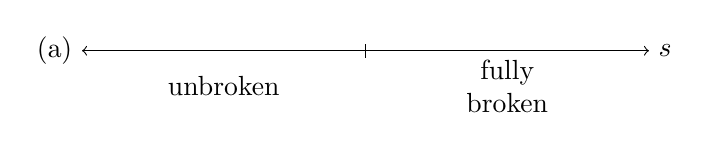
\begin{tikzpicture}[scale = .9]
\draw[<->] (0,0) node[left]{(a)}  -- (8,0) node[right]{$s$};
\draw (4,-.1) -- (4,.1);

\node [align=center] (A) at (2, -0.5) {unbroken};
\node [align=center] (C) at (6, -0.5) {fully\\broken};

\end{tikzpicture}
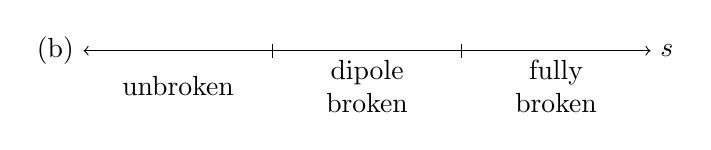
\begin{tikzpicture}[scale = .9]

\draw[<->] (0,0) node[left]{(b)}  -- (8,0) node[right]{$s$};
\draw (2.667,-.1) -- (2.667,.1);
\draw (5.333,-.1) -- (5.333,.1);

\node [align=center] (A) at (1.333, -0.5) {unbroken};
\node [align=center] (B) at (4, -0.5) {dipole\\broken};
\node [align=center] (C) at (6.667, -0.5) {fully\\broken};
\end{tikzpicture}

\caption{(a) For  $d>2$, there can be direct transitions between symmetry-unbroken and the fully-broken phase. Here $s$ is intended to represent a parameter along an arbitrary line in the phase diagram that crosses this transition. (b) At $d=2$, although the symmetry can be fully broken, the fully broken phase cannot touch the unbroken phase. Any line through the phase diagram that connects the two phases must pass though the dipole-broken phase. These phase diagrams are for translation invariant systems at zero temperature.}
\label{fig:phases}
\end{figure}

Let us now consider the same system, but with disorder.  The disorder Hamiltonian is
\begin{align}
H_\text{dis} &= \left[h_b\sum_j \sigma^*_jb_j + h_d \sum_{j,\mu} \sigma^*_{j,\mu}d_{j,j+\mu}\right] + H.C.,
\end{align}
where $h_b$ and $h_d$ control the magnitude of the disorder and each instance of $\sigma$ is a random phase. We will always consider $h_b,h_d<<1$.

At first, we will set $h_d=0$ but turn on $h_b$. This corresponds to the main considerations from Sec.~\ref{sec:disord}, where the disorder couples to the order parameter that fully breaks the symmetry. This raises the critical dimension for the superfluidity of the site bosons. The edge bosons may still enter a superfluid phase for $d>1$, but the site bosons may not condense with long range phase order until $d>4$. There cannot be a direct transition from the insulator to the monopole superfluid until $d>8$.  A phase akin to a Bose glass \cite{Fisheretal} of monopoles, where site bosons condense but without long-range order, can still exist in $1\le d<4$. 

Now, let $h_d\ne 0$ while keeping $h_b=0$. The Imry-Ma argument for the edge bosons says that they should not be able to enter a superfluid phase when $d\le 4$. Once again, we can enter a Bose glass phase where $\langle d_{j, j+\mu} \rangle \ne 0$. In this case, the site bosons acquire a random single particle {\it hopping}. This may be expected to give rise to a Bose glass phase also for the site bosons. This implies that the monopoles cannot even undergo mediated condensation to superfluidity for $d\le 4$. For $d>4$, the dipoles may enter a superfluid phase, and the monopoles can enter a superfluid phase without mediation.

It is difficult to justify including including one disorder field but not the other. The standard reason to forbid disorder is by imposing translation invariance, but if we are already including one disorder field we are necessarily breaking translation symmetry. For $h_b,h_d\ne 0$, we can fully rely on the Imry-Ma argument. No symmetry breaking can occur for $d\le 4$, the monopole superfluid must be separated from any symmetry-unbroken phase by a dipole superfluid for $4<d\le 8$, and any symmetry-breaking transition can occur for $d>8$. 

\section{Discussion} \label{sec:disc}

In this paper we analyzed the spontaneous symmetry breaking of various multipole groups, and discussed generalized Mermin-Wagner theorems, which (we argued) should be best understood as constraints on when a direct transition fully breaking a multipole group can occur, and when a symmetry unbroken phase and a (monopole) symmetry breaking phase must be separated by intermediate phases breaking higher multipole symmetries. We also considered multipole groups that are not the maximal multipole group, and the effect of quenched disorder. The disorder that we considered explicitly broke the symmetry, either fully or to a subgroup.

Of course, we could consider further combinations of effects. We could spontaneously break a symmetry from a group $G$ to a subgroup $H$ where either $G$ or $H$ are non-maximal. Or we could consider non-maximal groups with disorder. While the number of potential examples to consider is unlimited, they should all be analyzable using the ideas introduced herein. 

We should be clear that the arguments in this paper are Mermin-Wagner or Imry-Ma arguments. These essentially amount to stability analyses about the Gaussian symmetry breaking fixed point. In principle, even when the Gaussian symmetry breaking fixed point is unstable, a non-trivial fixed point with long range order could arise (see e.g. \cite{TonerRadzihovsky}). Whether and when such non-trivial fixed points can be realized in models with multipolar symmetry is an important problem for future work. 

We also emphasize that when the ordered phase does not exist, we did not provide any argument for what phase should replace it. For example, in 2 spatial dimensions there can be no ordered phases of continuous monopole (ordinary) symmetries. For $O(n)$ models with $n>2$, the result is that the disordered phase is the only phase \cite{polyakov}. For $n=2$, there can in addition be quasi-long-range-ordered phases. Determining what kind of phase {\it can} obtain in the absence of long range ordered symmetry breaking is beyond the scope of this work, and would at a minimum require understanding the nature and role of topological defects in the symmetry breaking order parameter, akin to vortices in the XY model. The range of possible symmetry unbroken phases could be even richer in the presence of disorder, where various glassy phases could also come into play \cite{Fisheretal}. Our discussion of disorder physics was also limited to quenched short-range correlated disorder. Extensions to disorder with long-range correlations, or annealed disorder, are left to future work.

We should also emphasize that our discussion has utilized standard concepts from statistical physics, which in turn amounts to assuming  ergodicity. However, quantum dynamics with multipolar symmetries can break ergodicity \cite{KHN, Sala}, in which case our analysis would not straightforwardly apply. It is however believed that the strict ergodicity breaking is limited to systems with strictly short range interactions (below some critical range) and that systems in which the interactions have long range tails (whether power law or exponential) should generically obey ergodicity at long times (although see \cite{NS}). Since long range tails are generic in physical systems, we believe our arguments should generically apply.  

Another setting for generalized Mermin-Wagner-type arguments is higher form global symmetries~\cite{GKSW, Lake, Marvin}. It would also be interesting to see what sort of subtleties could exist in the spontaneous breaking of those symmetries, through partial symmetry breaking or disorder. Since the order parameters for higher-form symmetries are nonlocal, it is difficult to couple disorder directly to the order parameters. In the case of arbitrary perturbations the symmetry becomes broken microscopically, but emerges at long wavelengths. Could disorder have any effect on the Mermin-Wagner behavior of higher-form symmetries? We leave these questions for future work. 

Finally, there exists a body of work on generalized Mermin-Wagner arguments in systems with subsystem symmetries \cite{Batista2005, SeibergA, SeibergB, SeibergC, Gorantla2021, Distler2021}. Subsystem symmetries are rather different in character to the multipolar symmetries discussed herein, but are also related to fracton phases via duality \cite{VHF2}. There can be theories with subsystem symmetries where symmetry breaking cannot occur even above the critical dimension, due to the UV/IR mixing~\cite{Gorantla2021}. However, it is always possible to write down theories that saturate the generalized Mermin-Wagner bound~\cite{Distler2021}.
Exploration of connections between the present work and the literature on subsystem symmetries would also be a fruitful topic for future work. 

{\bf Acknowledgements} This work was supported by
the U.S. Department of Energy, Office of Science, Basic
Energy Sciences, under Award \# DE-SC0021346

\bibliography{big}

\end{document}